%\chapter{Proposed -  The potentiation of memory and other complex features}
\chapter{Proposed -  Patterns in potentiation across multiple environments}
\label{chap:varying_environments}

\noindent
Authors: Austin Ferguson, Anselmo Pontes, and Charles Ofria

\noindent
Status: Proposed. %but all software has been developed as part of previous work.
%One environment comes from work that is currently only published as a chapter in Anselmo Pontes' dissertation \citep{pontesEvolutionaryOriginsCognition2021}. 
%The other environment is a variant of the Logic 9 environment used in Chapter \ref{chap:consequences_of_plasticity} to study plasticity. 
%I propose to study potentiation in two environments, both of which have been ported from Avida2 to MABE2 and are ready to be used. 
While data collection has not started, both environments I propose to explore have been ported from Avida2 to MABE2 and are ready to be used. 
%Part of this extension will focus on potentiation in the patch harvesting environment, looking at lineages that evolved the memory necessary to switch from consuming one patch to finding another. 
%This has all been implemented in Avida in MABE2, as well as the Logic 9 environment we use to replicate the plasticity environment seen in Chapter \ref{chap:varying_environments}.
% As we work to get the work ready to publish, I first re-implemented the system in the new, in-progress version of Avida with MABE2 and begun re-running all the data from the previous work. 
% My intellectual contribution is a deeper dive into the genotypes that heavily exploit a patch and then move on in search for a new patch. 
% While the previous work looked at one lineage, my plan is to look into \textit{all} lineages that exhibit this behavior. 
% Additionally, I plan to conduct analytic replay experiments on these lineages to see how the potentiation of patch-hopping behavior changed over time. 
 

\section{Introduction}

% Lead in - how does this relate to the other chapters
Previous work has shown that the environment can influence the relative contributions of adaptation, chance, and history \cite{smithFitnessEvolvingBacterial2022}. 
I have previously proposed testing how changes to the environment and underlying representation affect potentiation in successful lineages (Chapters \ref{chap:replaying_associative_learning} and \ref{chap:simplified_model}). 
However, I will be unable to concretely identify if differences between those two systems are due to changing the environment or the representation. 
To remedy this issue, here I propose to quantify potentiation along successful lineages in two additional Avida environments.
By keeping the representation constant, potentiation differences must therefore be a result of the change in environment or the targeted trait within. %due to the one factor that has changed, the environment. 

% The results of Chapters \ref{chap:replaying_associative_learning} and \ref{chap:simplified_model} are uncertain, but I expect one of three possibilities: %can have many potential outcomes, but we can boil them down to three categories: 
% 1) we observe similar patterns in potentiation between the associative learning Avida environment and the simplified bitstring model, 
% 2) potentiation looks drastically different between the two setups, with no discernible patterns, or
% 3) a mix, where some traits are shared and others are drastically different. 
% My hypothesis is that the third option is what we will observe. 
% However, regardless of which situation is true, the results of those chapters will lay the initial expectations for how potentiation varies as systems change. 
% Between those chapters I proposed to vary both the environment and the representation of organisms. 
% Here, I propose to lock the representation, analyzing potentiation in two additional environments within Avida. 

%Regardless of which situation is true, the results of those chapters will prompt us to look at the similarities and differences in potentiation between the two systems. 
%If there are differences, can we untangle \textit{why} these differences exist? 
%If the patterns are mostly the same, can we use this information to predict how potentiation will change when looking at other environments and target behaviors?
%These are the questions I propose to investigate in this chapter by looking at two different environments and target behaviors in Avida. 

%Avida has been used to study a wide variety of evolutionary dynamics, ranging from X to Y to Z. 

% Why stick with Avida? Easier comparisons with the same levels of epistasis. 
I hypothesize that in many cases, potentiating mutations are highly epistatic, as epistasis is one key way for a seemingly innocuous mutation to have a drastic effect on later mutations.
As such, studies of potentiation should employ representations capable of epistatic interactions. 
This is an advantage of using Avida; there are multiple possibilities for epistasis between instructions, and in previous work I have confirmed that these interactions are sufficient for complex potentiation dynamics (Chapter \ref{chap:alife_submission}).
By conducting studies of potentiation in multiple Avida environments, I will investigate how environmental differences influence potentiation as the underlying representation, and thus the potential for epistatic interactions, only slightly differ. 

%We have demonstrated in Chapter \ref{chap:alife_submission} that we can quantify how the potentiation of a target behavior changes along a successful lineage in Avida.
%By the time we start on this project, we will have observed potentiation at a larger scale (Chapter \ref{chap:replaying_associative_learning}) and in a simplified model (Chapter \ref{chap:simplified_model}). 
Specifically, I propose to investigate potentiation in a patch harvesting behavior and in phenotypic plasticity. 
In the patch harvesting environment described in \citep{pontesEvolutionaryOriginsCognition2021}, I will target the successful harvesting of multiple patches in an organism's lifetime. %memory usage in the decision to exploit the current patch or explore to find a new patch. 
In the cyclic logic 6 environment (Chapter \ref{chap:consequences_of_plasticity}), I will target optimal plasticity. 
%By changing the environments and the behaviors we consider successful, we will be analyzing very different fitness landscapes and the effects they have on potentiation. 
While both target behaviors are complex, their details differ both with each other and with associative learning from previous work (Chapter \ref{chap:replaying_associative_learning}). 
Ultimately, will these details influence how potentiation changes? 

% Expectations and impact
%Specifically, here we target two different yet related behaviors. 
The patch harvesting behavior I am targeting is a basic cognitive behavior. 
In order to harvest multiple patches, organisms must switch between exploring to find new patches or exploiting the patch they are currently on. % state in order to successfully harvest multiple patches. 
Similar to the associative learning behavior in Chapter \ref{chap:replaying_associative_learning}, this behavior requires several different components in order to function (information storage, memory retrieval and usage, etc.).
As such, I expect the two behaviors to exhibit similar patterns in potentiation. 
%Specifically, I expect that single mutations (especially in the formation and usage of memory) can result in a drastic potentiation increase. 
The other behavior, optimal plasticity in the cyclic logic 6 environment, is a reactive behavior that does not require memory. % has similarities and differences to the other two behaviors.
It does, however, still consist of multiple components (performing tasks and regulating them due to environmental cues) that can be neutral or deleterious in isolation. 
Therefore, I also expect to see similar patterns in potentiation in the evolution of optimal plasticity. % regardless of the difference in the behaviors. 

% Conclusion - this is important because regardless of what the outcome is, the information we gain will be incredibly useful for future studies into potentiation and the role of history in evolution
This work will expand upon the previous chapters, providing additional examples of how potentiation changes as we vary the environment and target behavior. 
All together, these works will shape how we view potentiation, and will provide an expanding dataset for other researchers to compare against in the future. 
% Note that this will be the first time incorporating what we learned from chapter 4?

% As we discussed in the previous chapters, we can quantify how potentiation, the likelihood a focal trait evolves from a given genotype, changes over time. 
% In those chapters, I proposed studying these changes in potentiation in the context of associative learning (Chapters \ref{chap:alife_submission} and \ref{chap:replaying_associative_learning}) and in a simple bitstring NK landscape model (Chapter \ref{chap:simplified_model}). 
% The goal of those chapters is to try and find common trends in how potentiation changes across multiple lineages. 
% Here we continue to expand on these questions by looking at potentiation of different behaviors in two other environments: microbial mat harvesting seen by early bilaterian animals and the classic Logic 9 Avida environment. 

% This chapter asks if the target behavior influences how potentiation changes over time given a fixed substrate (in this case Avida organisms). 
% We will conduct replay experiments on successful lineages from both environments, applying insights learned from the bitstring model of Chapter \ref{chap:simplified_model}, to see if any general patterns emerge. 
% If we do not see general trends in the evolution of different behaviors in Avida, that will be strong evidence that potentiation is very unique to the target behavior we are analyzing. 
% If we \textit{do} see general trends, however, this work (along with the previous chapters) will lay the groundwork for future studies in other environments, computational substrates, or even in living organisms. 
\section{Methods}

Here I describe the two environments and the behaviors that we are targeting within them. 

\subsection{The patch harvesting environment}

% What are we modeling?
The first environment aims to model the patch harvesting behavior of early bilaterians as they traversed microbial mats. 
Fossil records of the paths taken by these animals provide evidence of complex behavioral patterns, potentially resulting from early cognitive behaviors \citep{carboneWhenLifeGot2014}. 
This environment is a re-implementation of the one found in \citep{pontesEvolutionaryOriginsCognition2021}. 
In this environment, organisms are rewarded for consuming nutrients and punished for time spent off the patch. 
Here, we specifically look at environments with multiple patches of nutrients, and our target behavior is the successful consumption of multiple patches. 
This behavior requires switching between at least two tasks (exploring or exploiting), and as such, it is a cognitive behavior comparable to associative learning in Chapter \ref{chap:replaying_associative_learning}.
%This behavior requires memory to solve, and as such it presents a testbed for a cognitive behavior that is comparable to associative learning in previous work. 
%aim to quantify the potentiation of memory usage required to switch between exploiting one patch and exploring to find a new patch. 

% General overview of how the environment is used
Our Avida organisms exist in the typical 60x60 toroidal grid, with parent organisms replicating into a neighboring cell. 
The evaluation of the organisms, however, occurs on a toroidal, two-dimenstional spatial grid that represents microbial mats like those encountered by the early bilaterians. 
These environments consist of various patterns of nutrients that the organisms can consume and empty tiles whose traversal causes the organisms to waste energy. 

% How does the environment actually work?
To facilitate the consumption of nutrients, organisms are granted four new instructions to navigate their environment. 
Movement is accomplished via three instructions: \texttt{Turn Left}, \texttt{Turn Right}, and \texttt{Move Forward}. 
The right and left instructions rotate the organism 45 degrees in the appropriate direction. 
The move instruction always moves the organism a single tile in the direction it is pointing, including diagonally. 
Finally, the organisms are given a \texttt{Sense} instruction to pull information from their environment. 
Specifically, the sense instruction will give the organism a numeric cue depending on what floor tile it is currently on. 
%Nutrient tiles result in a 3 cue, while 
Empty tiles return a negative one, while already-consumed nutrient tiles result in positive one. 
Nutrients are consumed as the organism moves onto that tile without requiring an additional action, and as such organisms will never sense a nutrient tile that has not been consumed.  

% How does scoring work? 
Organisms are scored based on how well they consume nutrients and avoid empty tiles. 
The organism's score is increased by one for each nutrient consumed. 
For every empty tile visited, however, the organism's score is reduced by one to model the organism expending energy to move for no nutrient gain. 
Moving onto a previously-consumed tile has no effect on score, as if some residual nutrients could offset the energy consumption. 
Finally, as is often done in Avida, this score is used in an exponential. 
The performance of the organism is calculated as $2^{\text{score}}$, which means an additional nutrient consumed always doubles performance, regardless of how many nutrients have been consumed in total. 
As is customary in Avida, this score is used to weight which organisms receive the most updates and thus execute their genomes faster. 

\begin{figure}
    \centering
    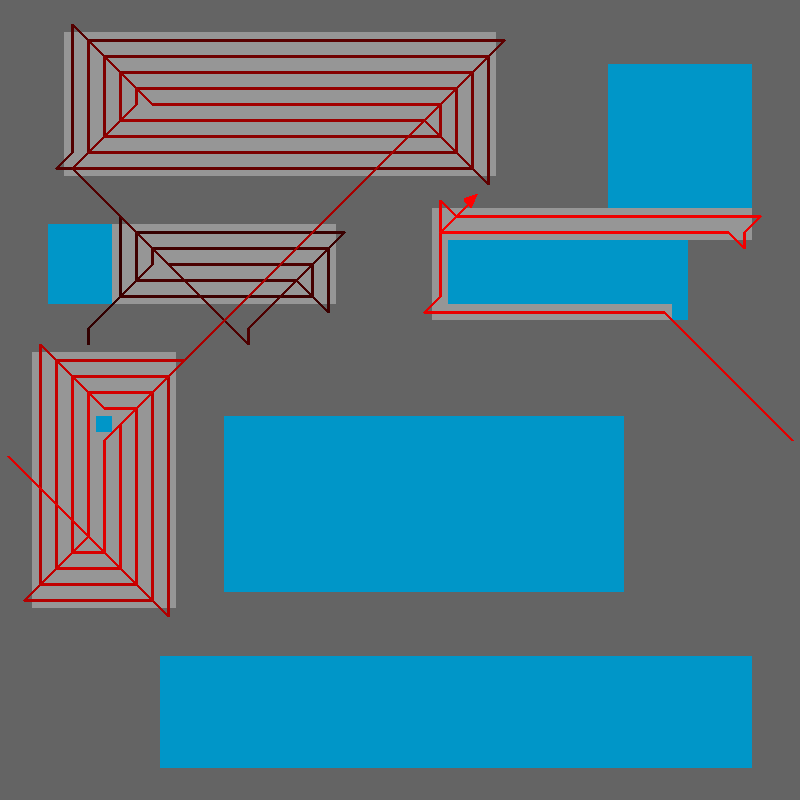
\includegraphics[width=0.9\textwidth]{06_memory_in_patch_harvesting/media/patch_harvest_example.png}
    \caption{
    An example layout of disconnected patches in the patch harvesting environment.
    Blue tiles represent food that has yet to be consumed, light gray tile are food that has been consumed, and dark gray tiles show empty space which is costly to move into. 
    The lines show the trace of an evolved organism (red triangle), with the start of the line in black and a slow fade to red as the trace becomes more recent. 
    This organism has evolved a spiraling behavior and has successfully consumed three patches of food. 
    }
    \label{fig:patch_harvest:example}
\end{figure}

% For more example images, see seeds 27, 31, and 32 for disconnected patches without edges

% Discussion of the target behavior and why it's cool
While previous work has used multiple patch types \citep{pontesEvolutionaryOriginsCognition2021}, here I propose to study only one: multiple disconnected patches.
The smaller patches in this environment require organisms to switch patches once they have exploited their current patch in order to maximize their score. 
These two behaviors (exploration and exploitation) can be thought of as two states the organism can be in.
As such, I expect this behavior to require memory, as a single bit of information is needed to store what state the organism is in. 
% The organism must determine when it has successfully consumed a patch and then move to find a new patch to eat. 
% This requires at least two states of behavior. 
Figure \ref{fig:patch_harvest:example} shows an example of the disconnected patches, as well as an evolved organism's successful trace through the environment. 
To easily categorize organisms that are capable of consuming multiple patches, I will require the organism to have consumed at least half each of two patches to be considered a ''successful'' behavior. 
Exploratory work has shown that this behavior does evolve, but only rarely. 
In 200 initial replicates, it appeared in only nine. % replicates. 
%This rarity works in our favor, as rare behaviors have the most room for potentiation gain. 
Much like associative learning in previous work, this rarity provides substantial room for improvements in potentiation over the course of a lineage. 

\subsection{The cyclic logic 6 environment}

% Intro
There may be inherent similarities between the associative learning task of Chapters \ref{chap:alife_submission} and \ref{chap:replaying_associative_learning} and the cognitive behavior needed in the patch harvesting environment. 
As such, here I propose one final, non-cognitive environment to test potentiation: the cyclic environment from Chapter \ref{chap:consequences_of_plasticity}, which I will refer to here as ``cyclic logic 6''. 

% Overview of environment
The cyclic logic 6 environment in Avida consists of two sets of bitwise logic tasks: one that is rewarded and one that is punished. 
Which set is rewarded, however, switches at regular intervals. 
Each organism receives a set of random input numbers, and then has the opportunity to perform computations and eventually output these values.  %performs whatever computation on them, and potentially outputs one or more values. 
If output values are deemed to be a successful logic operation on one or more inputs, then the organism is rewarded or punished according to the current state of the environment.  
The Avida organisms, however, are only given access to a bitwise \texttt{NAND} instruction, which they must use to build the other logic operations. 
% The simplest two tasks, NOT and NAND, confer a reward of 2, while we increase to a reward of 4 for AND and ORNOT, 8 for ANDNOT and OR, 16 for XOR and NOR, and finally a reward of 32 for EQU. 
% Rewards are multiplicative, so performing NOT and XOR would result in a performance of 32. 
% Organisms are only rewarded once for each logic task they perform. 

% Explanation of cycling
At any given time, three of the six logic tasks will be rewarded while the other three are punished. 
In this cyclic environment, this reward scheme is flipped at regular intervals.
%When this flip occurs, tasks that were rewarded become punished and vice versa. 
%An organism's score is doubled when it performs a rewarded task for the first time and halved when performing a punished task for the first time. 
When performing a logic task for the first time, an organism's score is doubled if that task is rewarded or halved if the task is punished. 
Here I flip the rewards and punishments every 100 updates. 
I will give organisms access to a new instruction, \texttt{Sense}, so they can determine what environment they are in and can potentially regulate task expression accordingly.
This environment is described in detail in Chapter \ref{chap:consequences_of_plasticity}, though here I am only using the PLASTIC environment from Phase 1 (see Figure \ref{fig:experimental-design}, panels A and C). 
I will use the same two sets of tasks used in Chapter \ref{chap:consequences_of_plasticity} (NOT, AND, and OR) and (NAND, AND-NOT, OR-NOT).

% What is optimal plasticity?
Due to the cycling of which tasks are rewarded, organisms must exhibit optimal plasticity to maximize fitness. 
As in the previous chapter, I define optimal plasticity as performing the three rewarded tasks and zero of the punished tasks. 
While organisms are born into a particular environment, I will test for optimal plasticity \textit{post hoc}, evaluating the organism in both variations of the environment. 
Therefore, for an organism to exhibit optimal plasticity, they must be capable of perfectly regulating all six tasks depending on which environment they are in. 

% Optimal plasticity is our target behavior
It is this optimal plasticity that I will target for the potentiation analysis. 
Compared to associative learning and multi-patch harvesting behaviors, optimal plasticity is a much more common behavior to evolve from the ancestor, with Chapter \ref{chap:consequences_of_plasticity} seeing greater than 40\% of replicates evolve the behavior.
While it is may be more common, this behavior is still nontrivial. 
To perform optimal plasticity, organisms must be capable of performing all six logic tasks, sensing the environment, and using the environment data to regulate the execution of the logic tasks. 
This task, however, can be solved reactively; it is unnecessary to store the environment state in memory. 
Still, I expect the complex nature of the environment to translate into interesting patterns in potentiation, not unlike those of associative learning seen in previous work. 



% Logic 9 has been well-studied in Avida. 
% Previous work has looked into how different evolutionary dynamics factor into the evolutionary dynamics of the more complex logic tasks, specifically equals (EQU) [CITE]. 
% As such, EQU provides us with a difficult-to-evolve target behavior that we can use for our potentiation studies. 
% By running analytic replays on lineages that evolve EQU, we can see how their likelihood to evolve the behavior changed over time. 
% This behavior has the potential to be quite different from associative learning from previous chapters or memory usage in the previous environment, as EQU does not require any cognitive processes. 
% Thus, the potentiation of EQU will be a solid basis of comparison as a behavior that does not require memory but is still difficult to evolve. 
\section{Proposed work}

In both environments, I will measure attributes of potentiation by conducting analytic replay experiments as described in Chapter \ref{chap:replaying_associative_learning}. 
I will then compare the measurements to previous data from Chapters \ref{chap:replaying_associative_learning} and \ref{chap:simplified_model} to determine what differences exist between the different environments. 
This work will provide additional examples of potentiation and allow the first cross-environment comparisons while keeping the underlying representation the same. 

Potentiation will be quantified using the exact same methods as Chapter \ref{chap:replaying_associative_learning}. 
Initial evolutionary replicates seeded with the default ancestor will be conducted to find replicates that exhibit the target behavior (multi-patch harvesting or optimal plasticity). 
For each environment, I will run initial replicates until I reach 40 successful lineages. 
To measure the changes in potentiation along the dominant lineage of each replicate, I will conduct two phases of replay experiments. 
The first will seed replicates with the genotypes found 50, 100, 150, and 200 steps before the target behavior first appeared in the lineage. 
I will continue to go backward along the lineage until a step shows less than 10 percentage points of improvement over the success rate from the initial replicates.
Once the exploratory replays have been conducted, I will identify potentiation windows (as in Chapter \ref{chap:replaying_associative_learning}) and seed replay replicates for every genotype in the windows. 
As before, I will run fifty replay replicates for each genotype analyzed. 

After conducting the replay experiments, I will collect the same potentiation measures described in Section \ref{sub:potentiation_measures}.
%These include maximum single-step potentiation gain/loss, the number of potentiation gain/loss windows, the fitness effect and behavioral background of potentiating/anti-potentiating mutations, and the distance between potentiating mutations and the appearance of the target behavior. 
Since these are the same measurements recorded in Chapters \ref{chap:replaying_associative_learning} and \ref{chap:simplified_model}, I can then statistically compare the distributions of each measurement across environments. 
The one exception is the behavioral background, which is unique to each task and thus can only be compared within a given environment. 
The cross-environment comparisons will be conducted first as a Kruskal-Wallis test to determine if significant differences exist across all of the environments \citep{kruskal_use_1952}. 
If a difference is detected, I will then conduct pairwise Mann-Whitney-Wilcoxon tests to look for significant differences between each pair of environments \citep{10.2307/3001968}. 
Finally, I will use a Holm-Bonferroni correction for multiple comparisons \citep{holmSimpleSequentiallyRejective1979}.

These comparisons will provide insight into how these potentiation dynamics vary when the environment changes but the representation stays the same. 
I expect only small differences between the associative learning behavior of Chapter \ref{chap:replaying_associative_learning} and the patch harvesting behavior examined here. 
Both cognitive behaviors require memory and have exist in environments containing non-cognitive alternative behaviors with high performance that might function as local optima. 
For the other environment, cyclic logic 6, I expect to see similar overall dynamics but a difference in the measured values. 
While the environment and behavior are drastically different from the other two, one particularly notable difference is that $>40\%$ of replicates evolved optimal plasticity in the different experiments of Chapter \ref{chap:consequences_of_plasticity}. 
Therefore I do not expect the same levels of potentiation gain as we observed in the evolution of associative learning in Chapter \ref{chap:alife_submission}, simply because the lineages start with a much higher level of potentiation. 
%Alternatively, lineages could still experience these  most of their potentiation in a single mutation, or we could observe more potentiation losses in this environment. 
Alternatively, we must consider that the cyclic logic 6 environment is the only proposed environment that changes with time; these changes to selective pressures may repeatedly break down potential building blocks and thus increase the potentiation gain when they are finally utilized. 
Regardless of the outcome, this work will provide needed data on potentiation and more insight into how evolution is (or is not!) contingent on initially innocuous mutations. 
